\vspace{0.015\textheight}
Missing energy is one of hardest kinematic quantities to understand because its measurement is a convolution of many effects. Missing energy is a powerful tool for SM and BSM physics searches, but its use is often hindered by the QCD background (fake \met). The reconstruction of \met is described in Section~\ref{sec:MetReconstruction}.

\begin{singlespace}
Possible sources of fake missing energy include:
\begin{enumerate}
 \item Calorimeter energy mismeasurements
 \item Unclustered energy (calorimeter energy not included in any of the reconstructed objects)
 \item How the objects are reconstructed (the clustering method)
 \item Wrong vertex selection
 \item Beam-related effects
 \item Objects lost in the uninstrumented regions
\end{enumerate}
\end{singlespace}

The conventional means of removing fake \met sources involves rather blind selection requirements. They are blind in the sense that they do not consider event topology and do not use an in-situ analysis of the event. For example, requiring \metg{20} is one such selection requirement. If an object in an event is badly mismeasured, the \met could easily fall below or rise above this threshold. Another example is a $\Delta \phi$ separation requirement between the direction of the \met and other objects in the event. In either of these situations, sensitivity is lost for new physics with moderate \met or particles produced close to the \met direction.

A method known as the ``Missing Energy Resolution Model'' (or \met Model) attempts to efficiently separate events with true and fake \met while remaining sensitive to new processes with \met as low as 20~GeV \cite{cdfnote:9184}. This method has been successfully used in several other analyses.

\section{\met Model}
The standard MET significance is defined as \met-sig = \met/$\sum \et$. However, fake \met depends on how the energy is distributed. The diagrams in Fig.~\ref{fig:FakeMetTopologyDependance} explain the amount of fake \met and depend on how the energy is distributed in the event. When the objects in the event, specifically jets, are uniformly distributed in $\phi$, the mismeasurement effects tend to cancel out. However, in the situation depicted in the rightmost diagram, the mismeasurement of jets would give rise to a significant amount of fake \met in a preferred direction.

\begin{figure}[htb!]
 \centering
 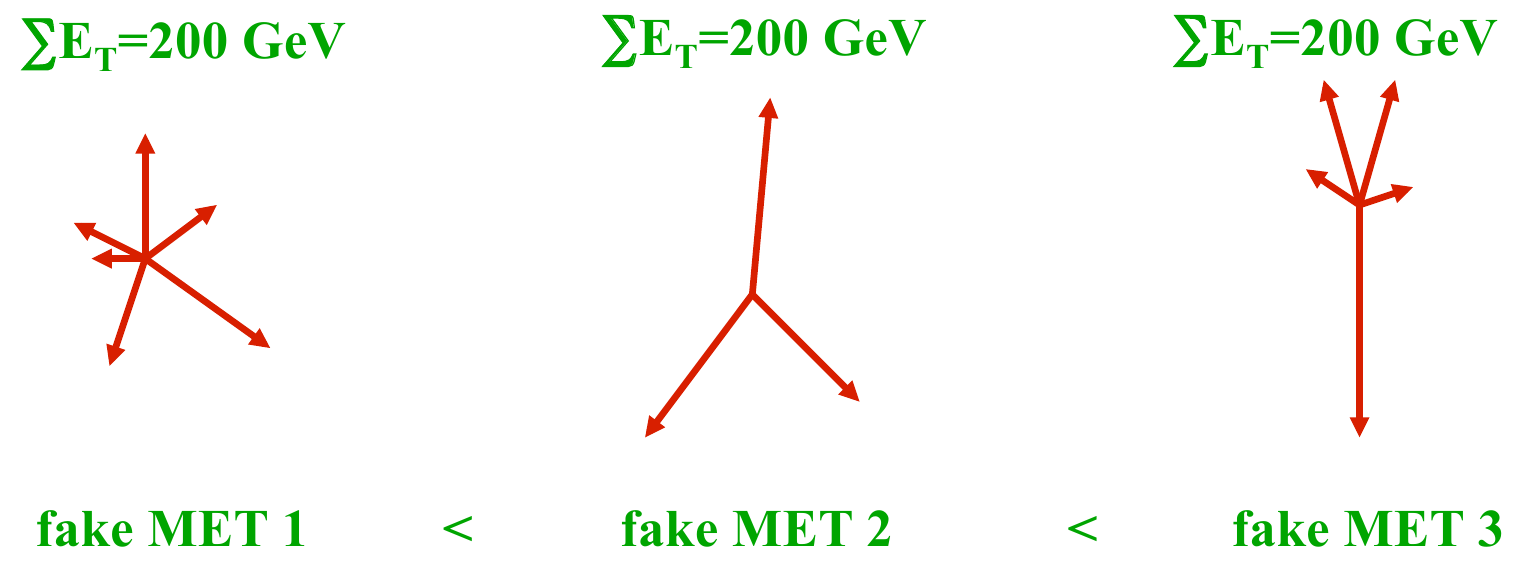
\includegraphics[scale=0.3,keepaspectratio=true]{./MetModel_fakeMET_topologicalDependence.png}
 % MetModel_fakeMET_topologicalDependence.png: 1537x564 pixel, 96dpi, 40.66x14.92 cm, bb=0 0 1153 423
 \caption[Dependence of fake \met on the distribution of energy in an event.]{Dependence of fake \met on the distribution of energy in an event. These three event topologies have a total $\sum\et$ of 200~GeV.}
 \label{fig:FakeMetTopologyDependance}
\end{figure}

This method attempts to address two major sources of fake \met: the mismeasurement of clustered energy (jets) and the mismeasurement of soft unclustered energy from the underlying event or multiple interactions. The \met model assumes that the fake \met is the vector sum of \met from these two components.

The unclustered soft energy tends to occupy the calorimeter rather uniformly and hence its overall contribution to fake \met is relatively small. To measure and quantify the fake \met due to unclustered energy, the contributions from the raw energies of all photons and electrons and all jets with $E_{T}^{lev6}\geq 15$~GeV are subtracted from the raw \sumet, which is calculated with respect to the highest \sumpt vertex. A parameterization is derived from \zee and di-photon \MC events, which have no intrinsic \met. The $x$ and $y$ components of the fake \met are parameterized by a double gaussian as a function of $\sqrt{\sum E_{T}}$:
\begin{equation}
 F(\met_{X,Y})=\frac{G(mean,\sigma)+Norm\times G(mean,scale\times\sigma)}{1+Norm}
 \label{eqa:MetModel_UnclParameterization}
\end{equation}

\begin{figure}[h!]
 \centering
 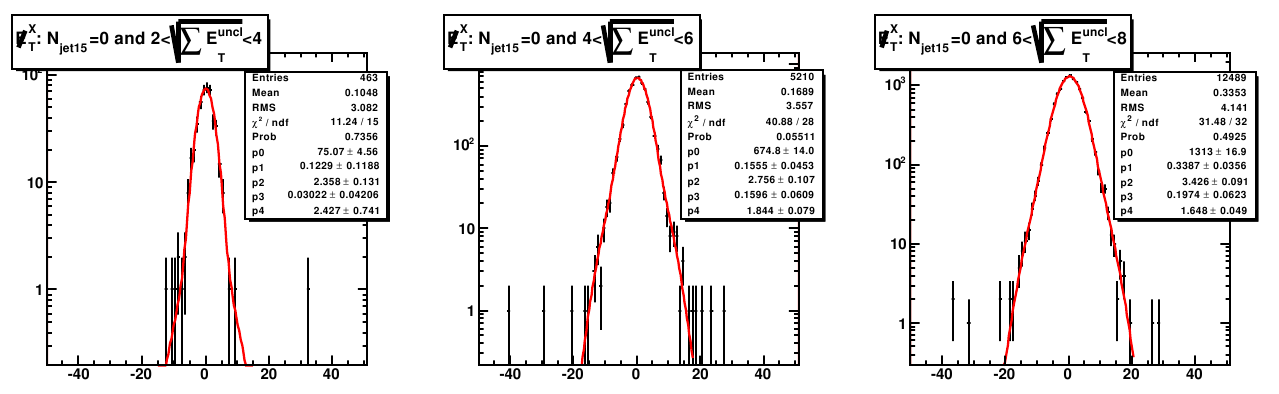
\includegraphics[scale=0.4,keepaspectratio=true]{./MetModel_UnclParameterization.png}
 % MetModel_UnclParameterization.png: 1279x394 pixel, 96dpi, 33.84x10.42 cm, bb=0 0 959 295
 \caption{Paramaterization of unclustered energy in bins of $\sqrt{\sum E_{T}}$.}
 \label{fig:MetModel_UnclParameter}
\end{figure}

The mismeasurement of clustered energy (jets) is the largest source of fake \met and it affects the direction of \met greatly. To reduce this effect, the raw \met (\metRaw), measured with respect to the highest \sumpt vertex, is corrected using the highest \sumpt vertex position. Then the \met is adjusted for the presence of any jet with corrected energy \etg{15}. The \met correction due to an individual jet is described by
\begin{equation}
 \mbox{\metCorrVec} = \vec{\met} - (\vec{E}_{T}^{lev5}+\vec{MI}-\vec{E}_{T}^{raw})=\vec{\met}-\vec{E}_{T}^{lev5}-\vec{E}_{T}^{lev1}+\vec{E}_{T}^{lev4}+\vec{E}_{T}^{raw}
 \label{eqa:MetModel_JetCorrection}
\end{equation}
\noindent where \metCorrVec is the missing transverse energy corrected for a jet, \metVec is the missing transverse energy before correcting for this jet, $\metVec^{lev5}$ is jet energy corrected to level 5, $\vec{MI} = \metVec^{lev1} - \metVec^{lev4}$ is the contribution due to multiple interactions, and \metRaw is the raw jet energy before any corrections.

This process is repeated for all the jets in a event with $E_{T}^{lev6}\geq 15$~GeV.

To account for a jet's contribution to \met, the jet energy resolution ($JER$) is derived as a function of the jet's energy ($E$) and pseudorapidity ($\eta_{det}$) using dijet Monte Carlo data. The jet energy resolution is defined as the ratio of detector- and hadron-level\footnote{Hadron-level jets are reconstructed similarly to detector-level jets by including all hadronized particles in a cone of radius 0.4} energies, $JER = E^{det}/E^{had} - 1$. The behavior of the jet energy resolution as a function of the transverse energy of the jet is shown in Fig.~\ref{fig:MetModel_JERwithJetEt}. Hadron-level jets and detector-level jets are matched within a cone of $R(\phi,\eta)<0.1$. The $JER$ is derived in bins of 5~GeV of jet energy and $\eta$ bins of $\Delta\eta_{det}=0.2$. A set of sample $JER$ distributions is shown in Fig.~\ref{fig:MetModel_JERforEtEtaBin}. Each of these $JER$ is assumed to be described by a combination of a Gaussian and Landau distribution:
\begin{equation}
F(x) = \frac{C\times Gauss(-x/(1+x))+Landau(-x/(1+x))}{C+1}, ~~~ x=\frac{E^{det}}{E^{had}}-1
\label{eqa:JER}
\end{equation}
To simply the implementation, the Gaussian and Landau parameters from individual fits from each ($E^{jet},\eta_{det}$) bin are extracted and parameterized as a function of the energy of the jet. Similarly, a relative normalization ($C$) is also derived. These parameters are fitted with the following function of $E^{jet}$ for each $\eta$ bin.
\begin{eqnarray}
Gaussian~and~Landau: \sigma &=& \sqrt{\frac{p_{0}}{E}+p_{1}}\\
Gaussian~and~Landau:~mean,~mpv &=& p_{0}+p_{1}E+p_{2}/E\\
C&=&\frac{p_{0}+p_{1}\sqrt{E}}{E}+p_{2}
\end{eqnarray}


\begin{figure}[htb!]
 \centering
 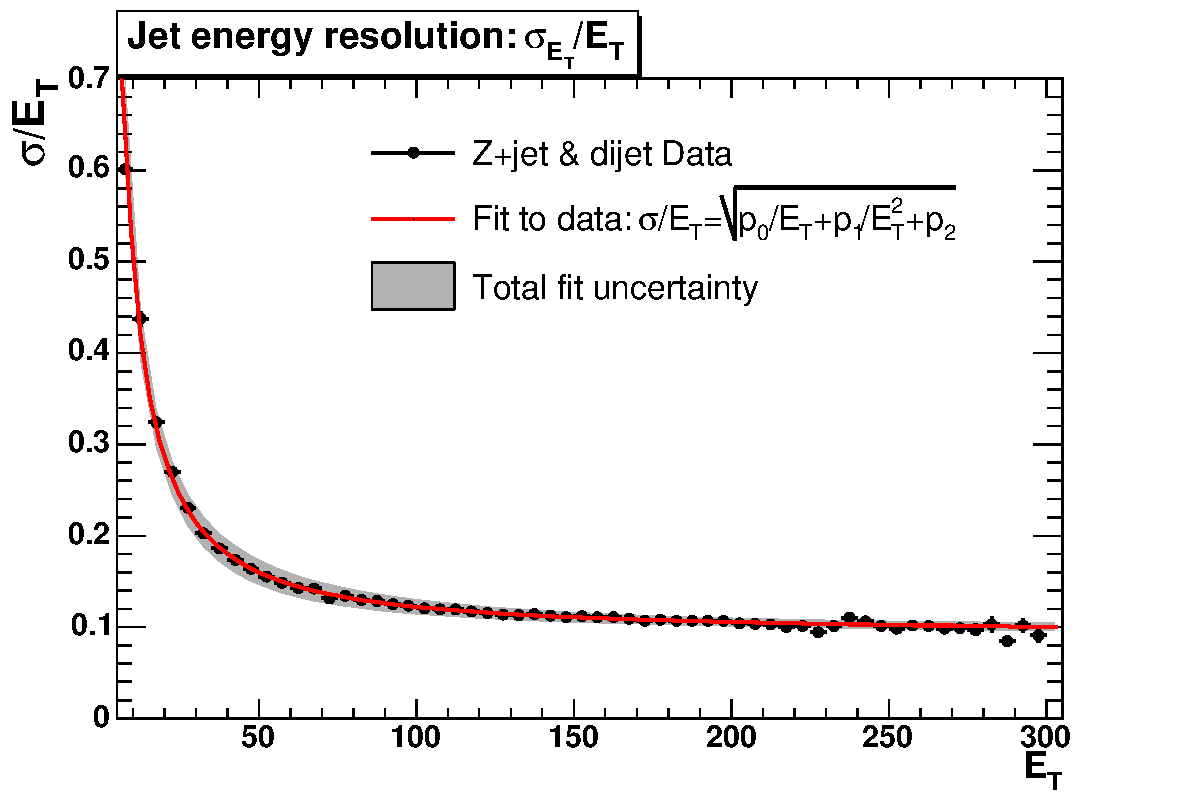
\includegraphics[scale=0.6,keepaspectratio=true]
{./MetModel_JER.pdf}
 % MetModel_JER.pdf: 612x792 pixel, 72dpi, 21.59x27.94 cm, bb=0 0 612 792
 \caption{Jet energy resolution as a function of jet energy.}
 \label{fig:MetModel_JERwithJetEt}
\end{figure}

\begin{figure}[htb!]
 \centering
\subfigure{
 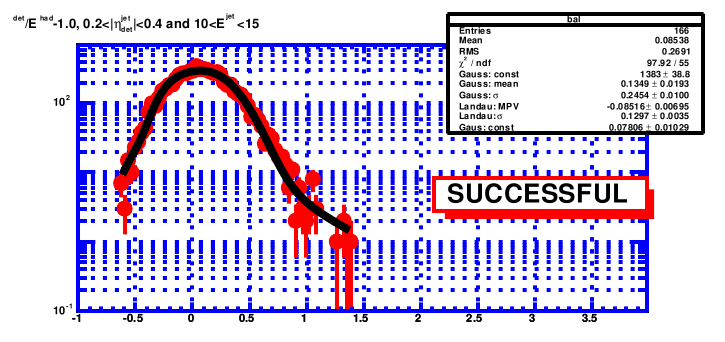
\includegraphics[scale=0.6,keepaspectratio=true]{./MetModel_Jer1.png}
}
\subfigure{
 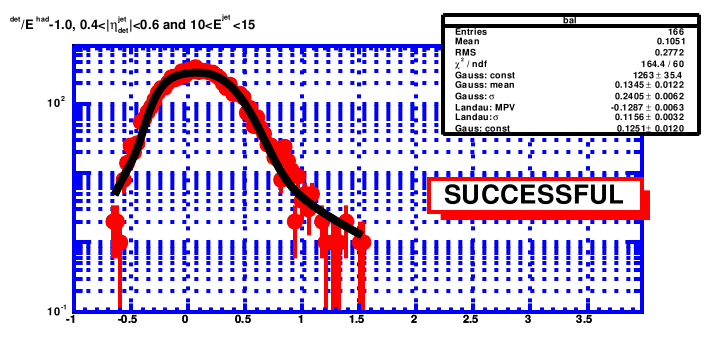
\includegraphics[scale=0.6,keepaspectratio=true]{./MetModel_Jer2.png}

}
\caption{Parameterization of the jet energy resolution in jet $\eta$ and energy.}
\label{fig:MetModel_JERforEtEtaBin}
\end{figure}

These energy resolution functions are used to predict the shape of the fake \met. For every event, a probability distribution function of fake \met, ${\cal P}(\met)$, is generated by smearing energies of all objects (jets and unclustered energy) in the event. The smearing is done according to objects' energy resolution functions and generating large number of pseudo-experiments. Summing up the individual ${\cal P}(\met)$ distributions for all events provides a shape of the predicted fake \met due to energy mismeasurements.
% Figure xxx demonstrates a comparison of observed and predicted by the Met Model \met-distribution in \pythiaText $\gamma\gamma$ and \zee events. [TODO: INCLUDE SIMILAR FIGURES FROM g+jets MC (and DATA??)]
The details of calculating ${\cal P}(\met)$ are explained next.

For a given event, for each pseudo-experiment, all jets with \etg{3} and \etalessthan{3.0} are smeared according to $JER(E^{jet},\eta_{det})$ as defined in Eq.~\ref{eqa:JER}. If any jet's smeared energy, $E_{T}^{smear}$, is above a 15~GeV/$c$ threshold, its contribution to \met is calculated as:
\begin{equation}
 \vec{\met}^{jet,i} = \vec{E}_{T}-\vec{E}_{T}^{smear}
\label{eqa:MetSmearing}
\end{equation}
This is done as a vector sum of all $\vec{\met}^{jet,i}$. By doing so, the direction of jets with respect to the \met direction is taken into consideration. This means a jet perpendicular to the direction of the \met could not have contributed to fake \met. Any other jet would have varying contributions, while a jet along or directly opposite to the \met direction will have the largest contribution to the fake \met.

If a jet fluctuated below the 15~GeV threshold after smearing, the unclustered energy based on $E_{T}^{smear}$ is recalculated. Then, a new expected $\met_X$ and $\met_Y$ are randomly generated to calculate the unclustered component of the fake \met using Equation~\ref{eqa:MetModel_UnclParameterization}.

Finally all the individual \met components due to the soft unclustered energy and each of the jets with $E_{T}^{smear}>15$~GeV are added together to obtain the final prediction of fake \met.

The \met model is not designed to predict the exact value of \met in each event. Instead, it provides the most likely distribution of \met which can arise due to energy mismeasurement in the calorimeter. The \met model can also provide an event-by-event probability, ${\cal P}(\met)$, that measures the probability of obtaining a particular value of \met entirely due to fluctuations in energy measurements. This probability distribution function can also be used to calculate the significance of the measured \met (\met-significance or \met-sig). Choosing a suitable \met-significance value allows one to select or remove a certain number of events with fake \met in order to model the remaining fake \met distribution.

% TESTS PERFORMED AND CONCLUSION:
% \section{TODO: EXCLUSIVE 1 JET RESULTS}
% \section{TODO: IMPROVE JET PARAMETERIZATION}
% \begin{figure}[htb!]
% \centering
% 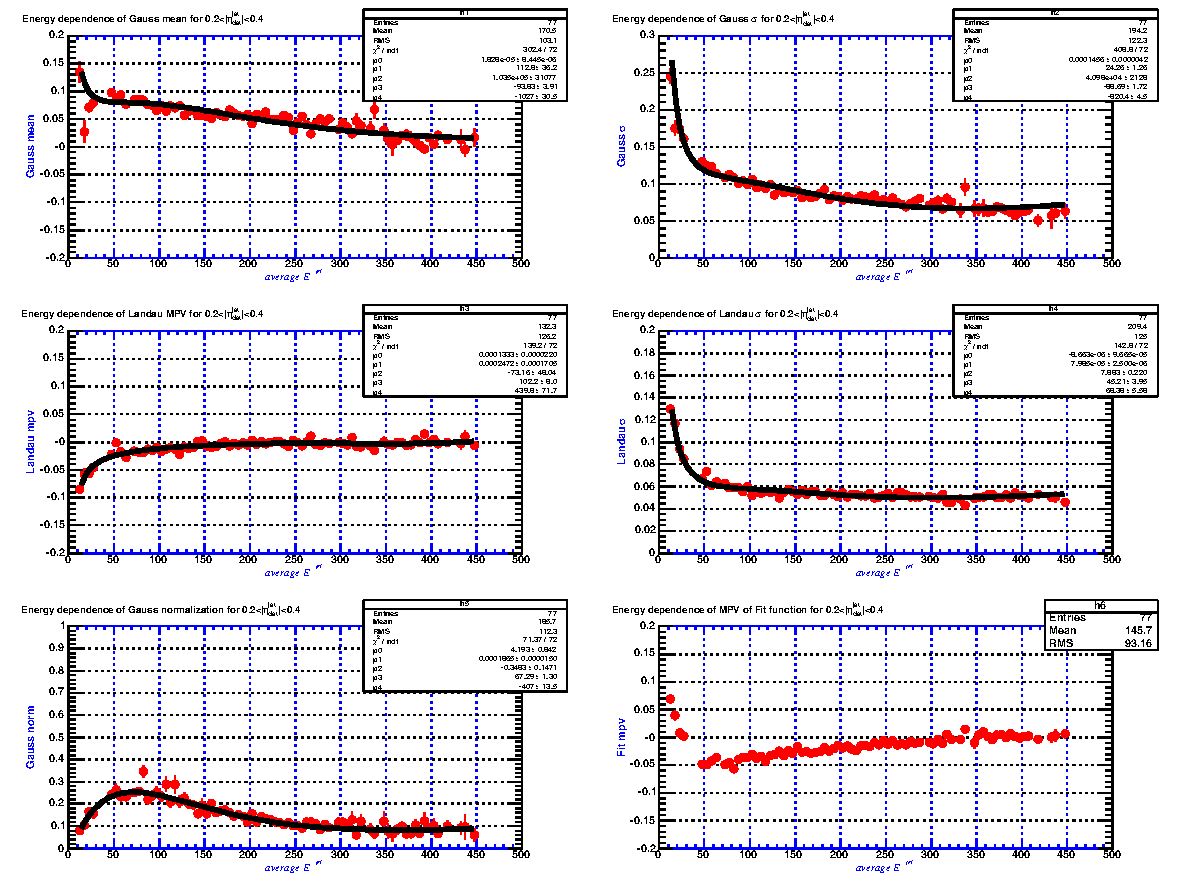
\includegraphics[scale=0.75,keepaspectratio=true]{./MetModel_JERfit_EtaBin1.pdf}
% % MetModel_JERfit_EtaBin1.pdf: 567x425 pixel, 72dpi, 20.00x14.99 cm, bb=0 0 567 425
% \caption{Sample plot showing JER fit for a eta bin.}
% \label{fig:MetModel_JERfit}
% \end{figure}
%
% \section{TODO: Photon Energy Resolution}
% Photon energy resolution is investigated in order to check its significance on the final predictions.
%
% \begin{figure}[htb!]
% \centering
% \subfigure{
% 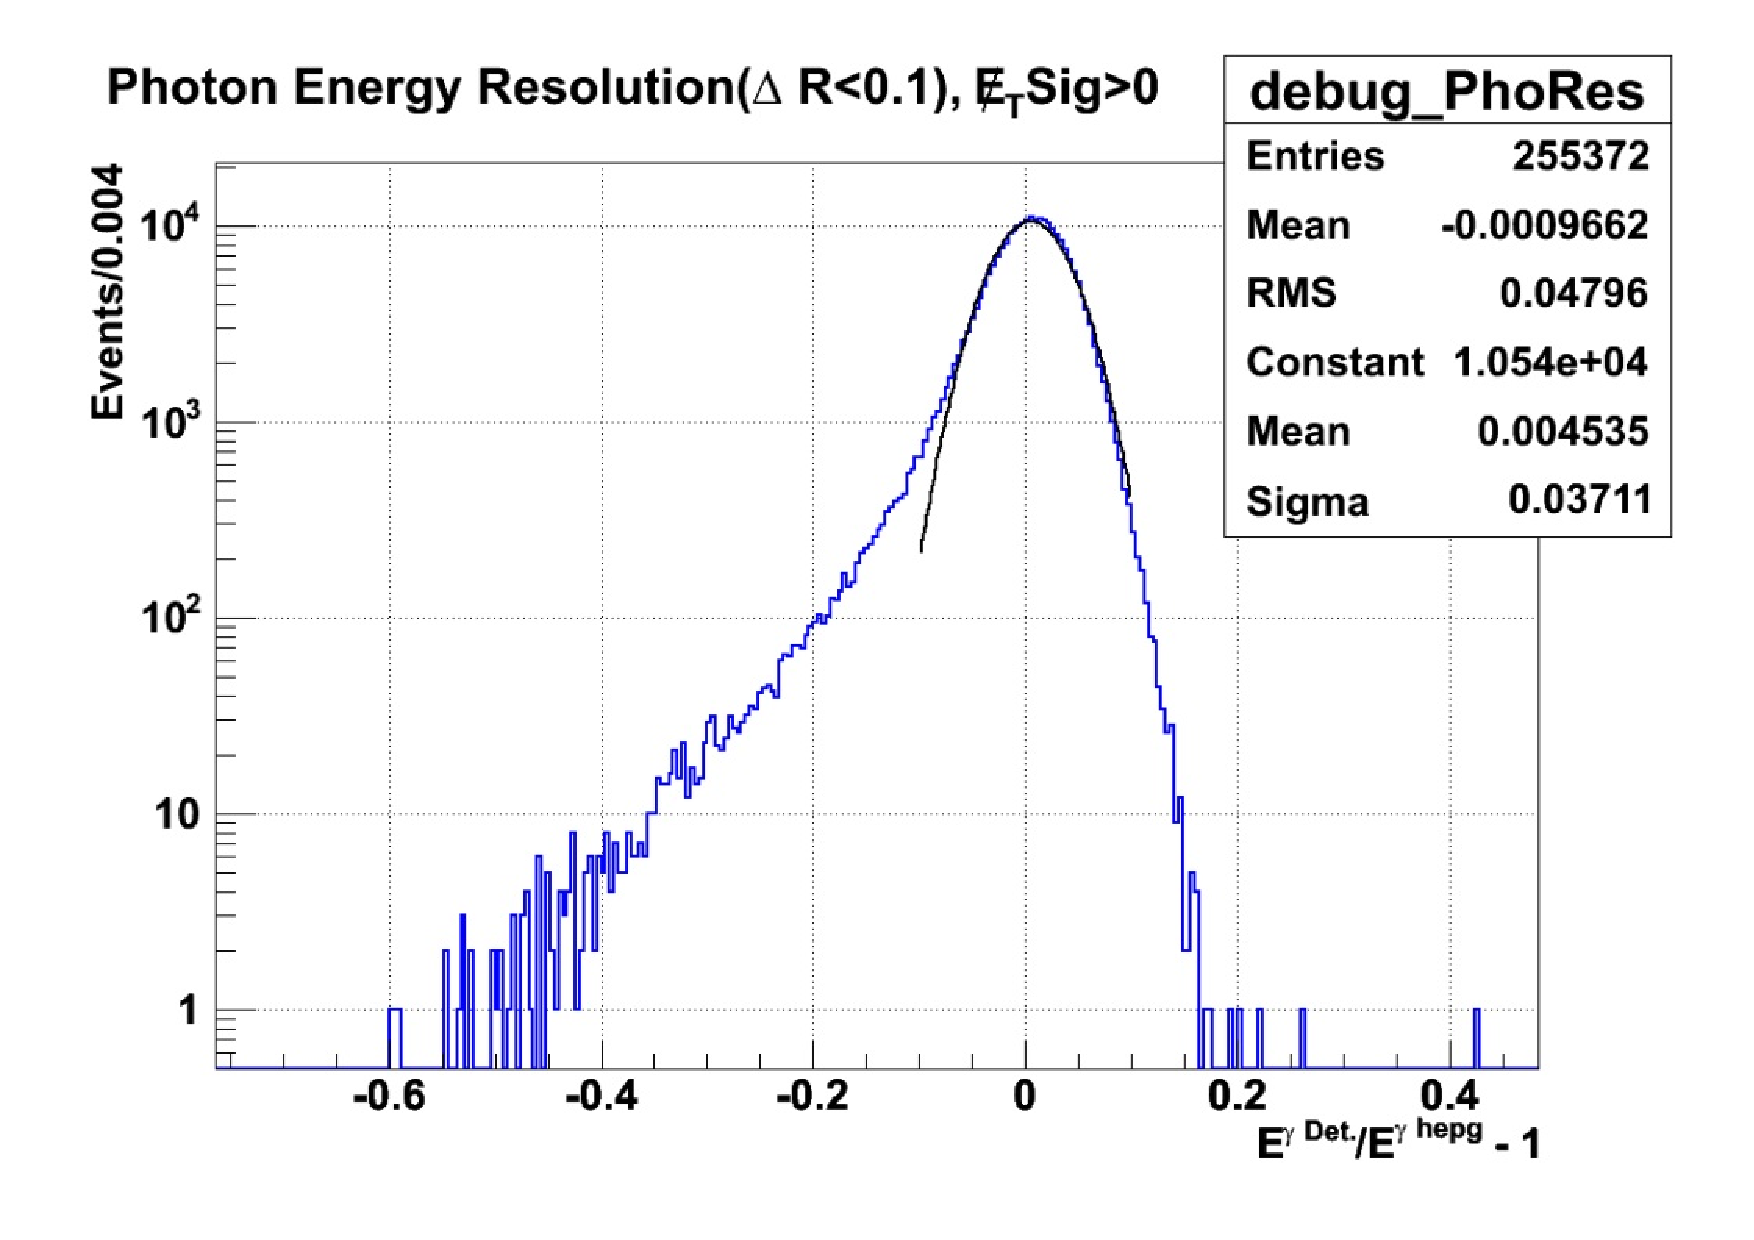
\includegraphics[scale=0.25]{./MetModel_PhoRes_MetSig0.pdf}
%
% 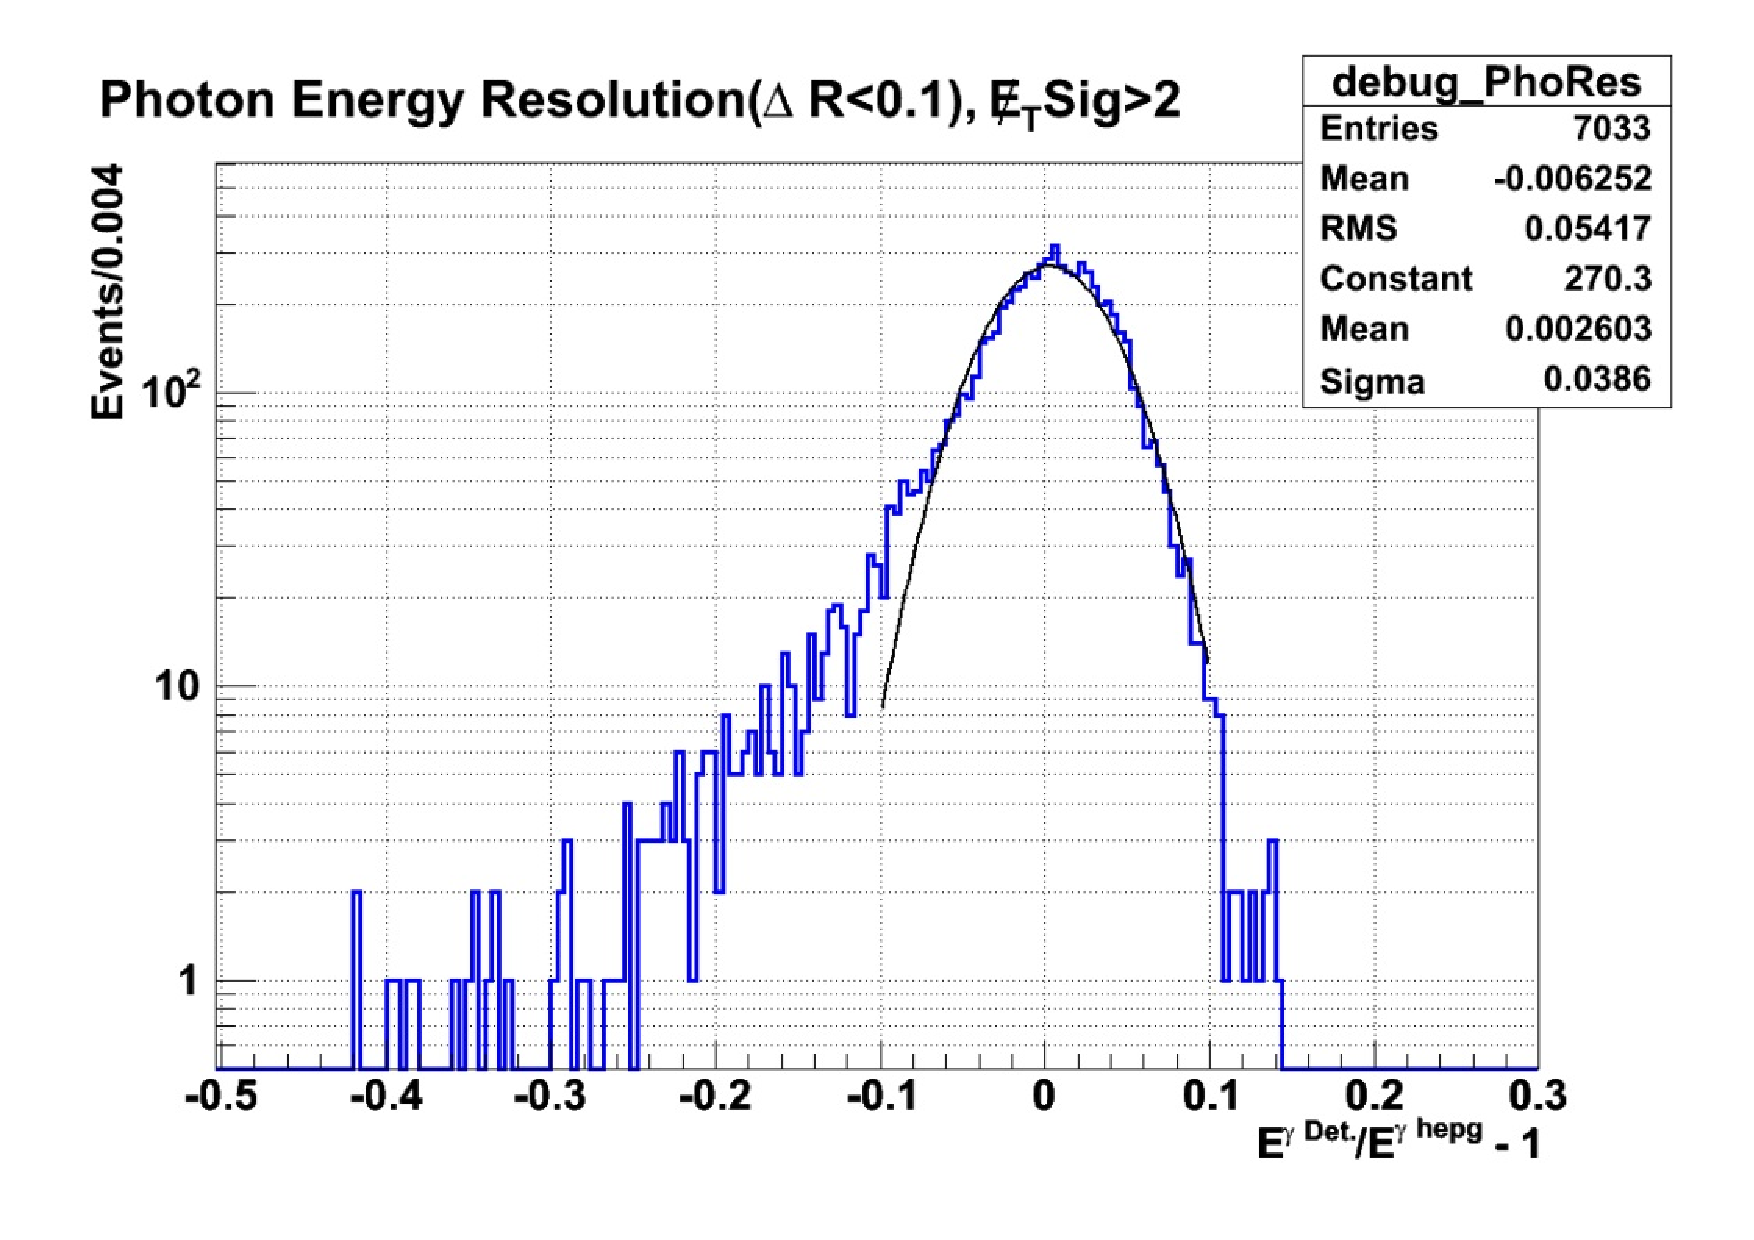
\includegraphics[scale=0.25]{./MetModel_PhoRes_MetSig2.pdf}
% }
% \caption{Photon energy resolution for different \met-sig.}
% \label{fig:MetModel_PhoRes}
% \end{figure}
%
%
% \section{TODO: MET ADDITION TO JETS: leading jet}
% \section{TODO: DOUBLE SMEARING EFFECT}.
% \begin{figure}[htb!]
% \centering
% \subfigure{
% 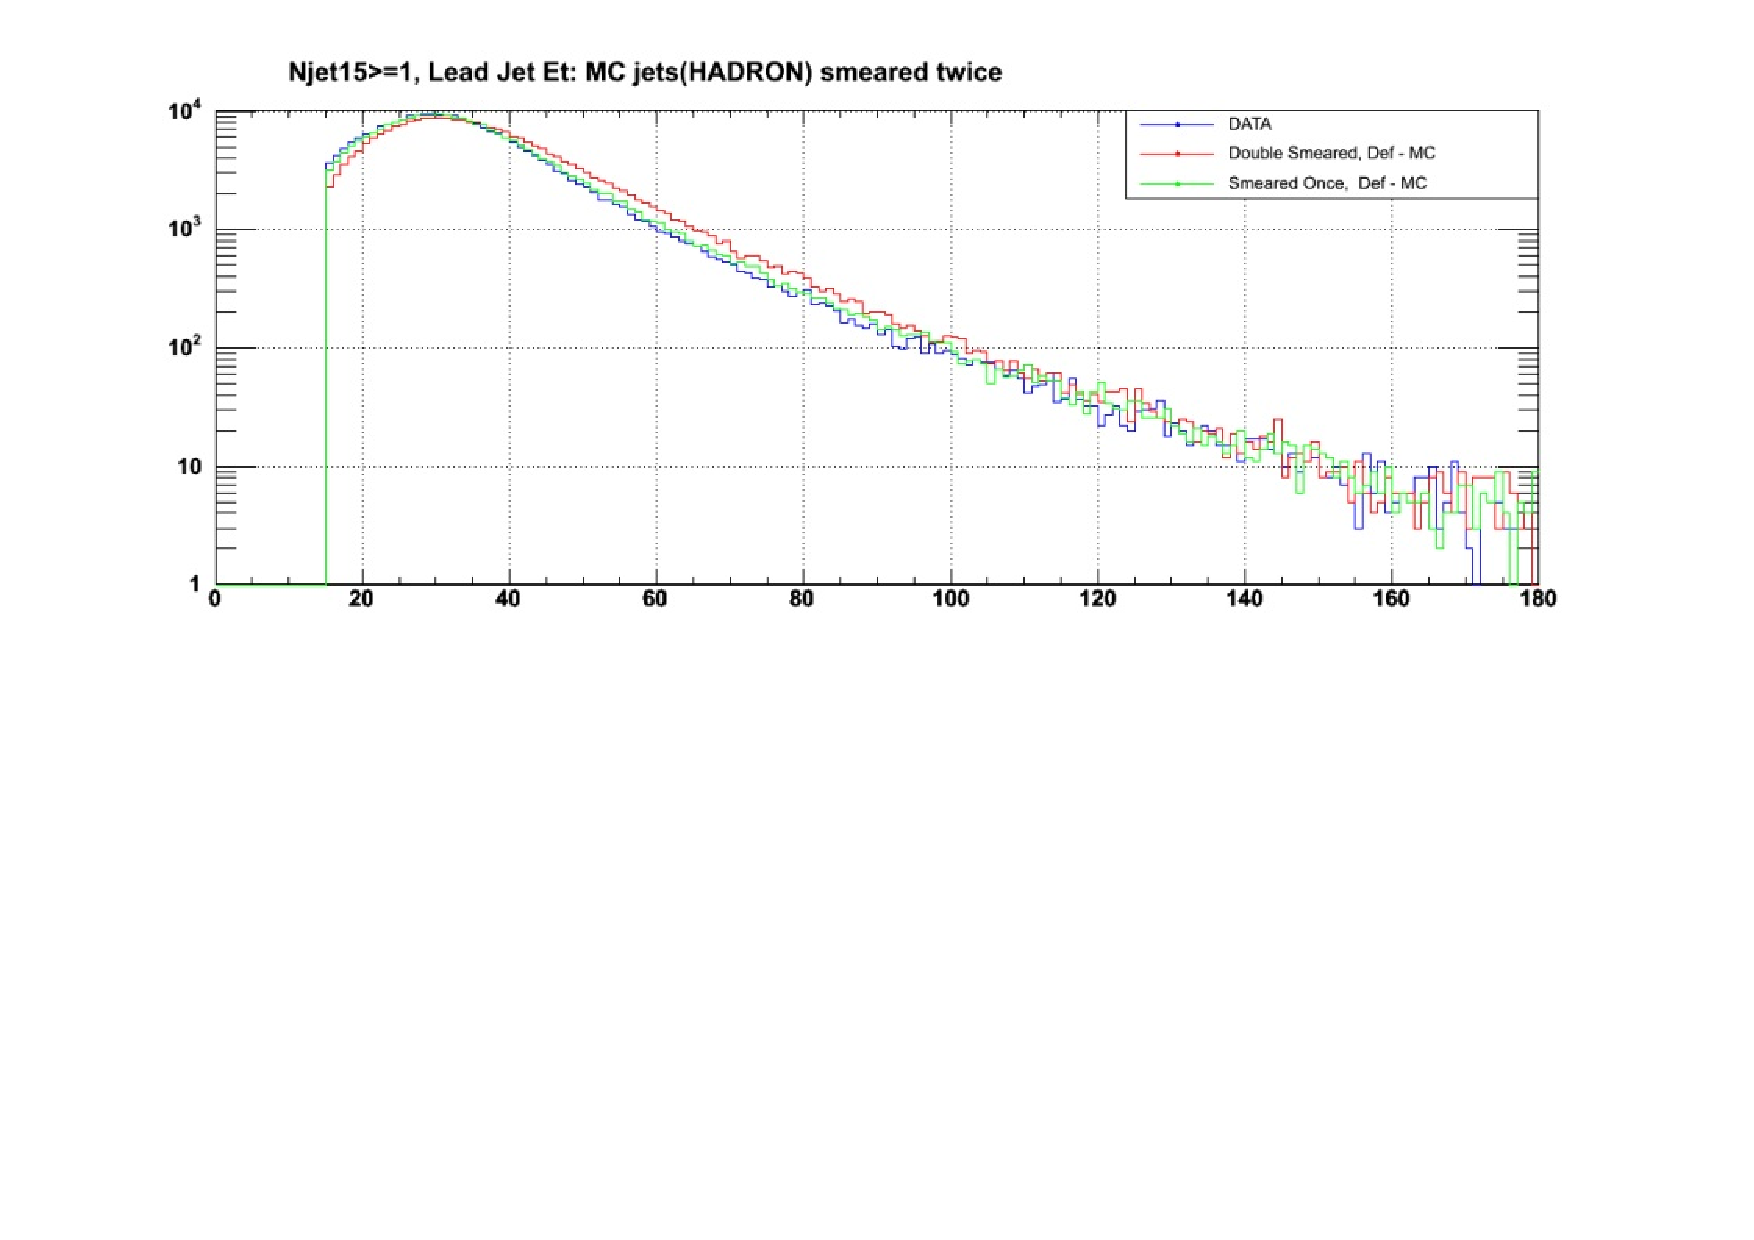
\includegraphics[scale=0.3,keepaspectratio=true]{./MetModel_DoubleSmear_JetEt.pdf}
% }
% \subfigure{
% 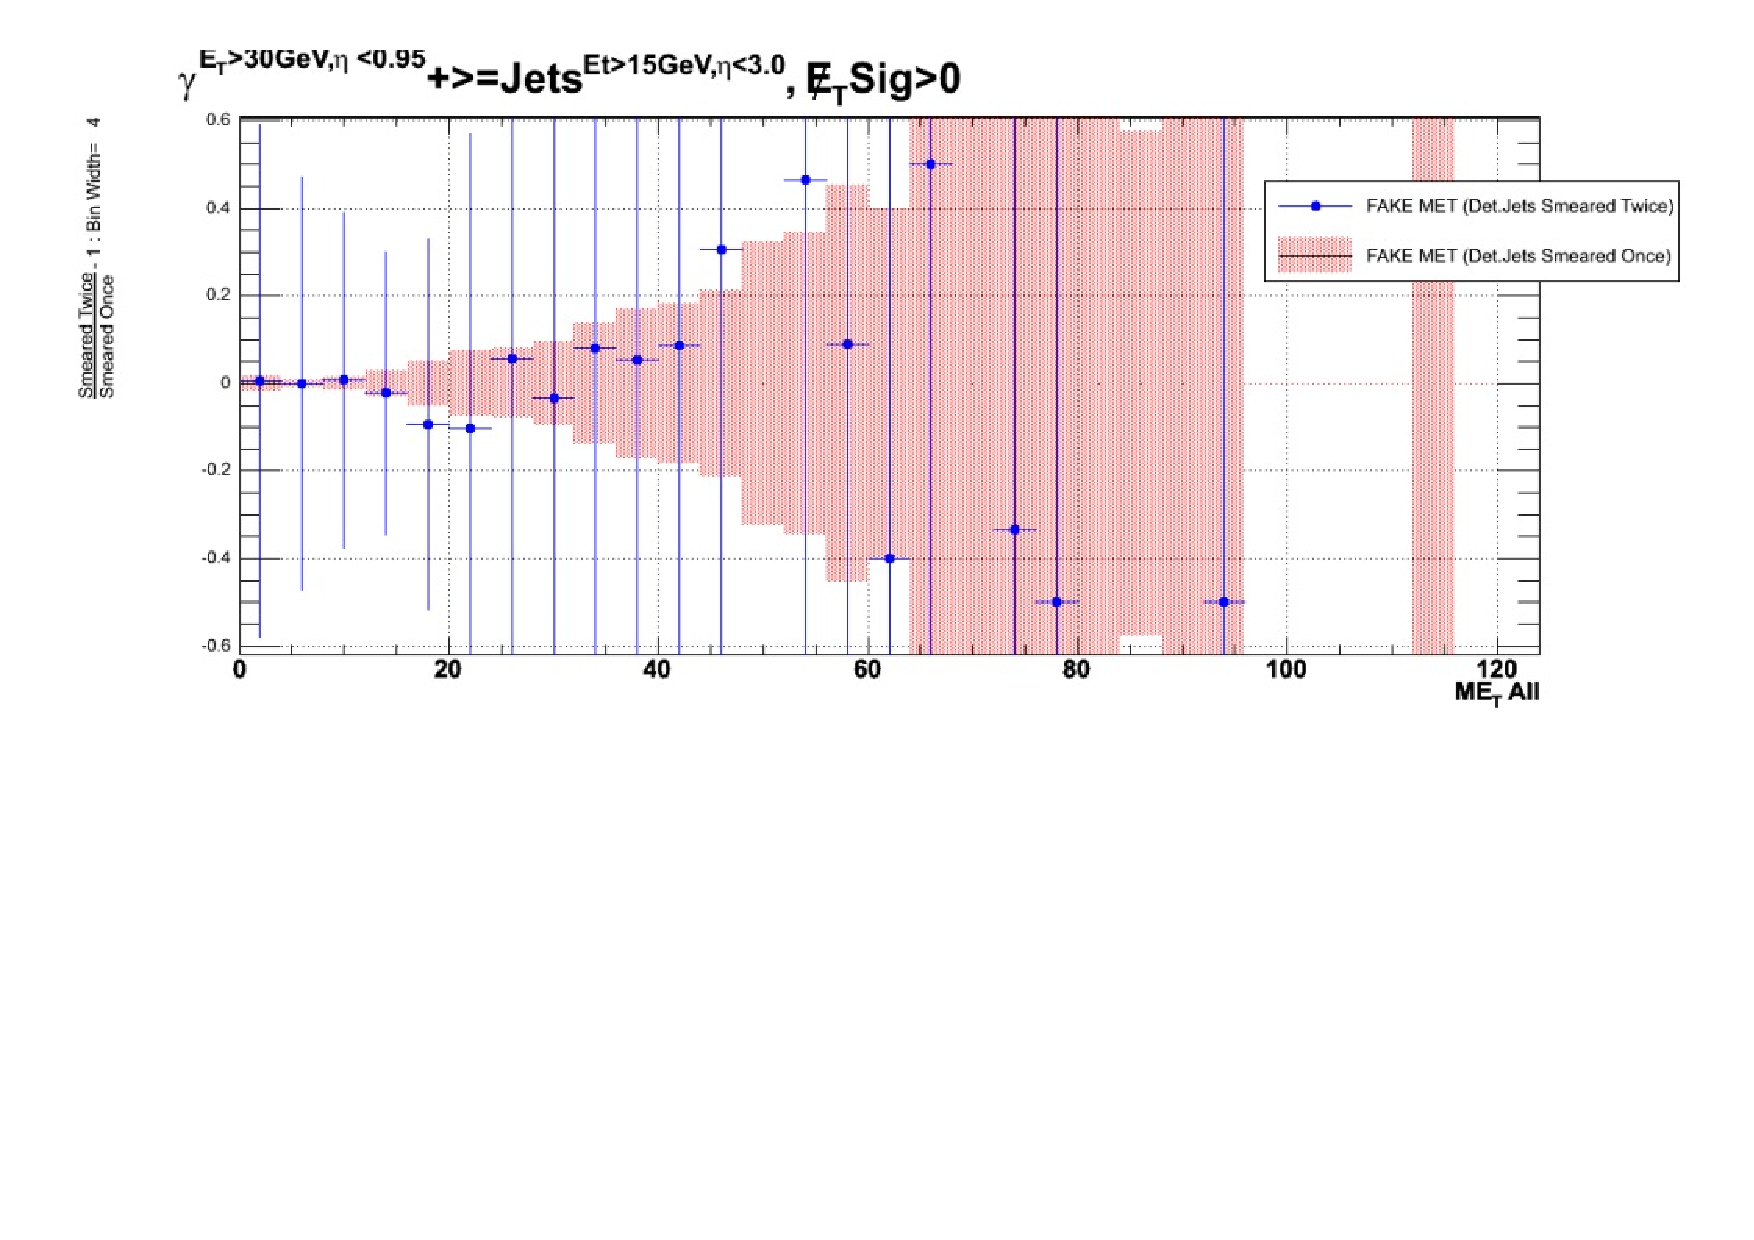
\includegraphics[scale=0.3,keepaspectratio=true]{./MetModel_DoubleSmear_MetAll.pdf}
% }
% \subfigure{
% 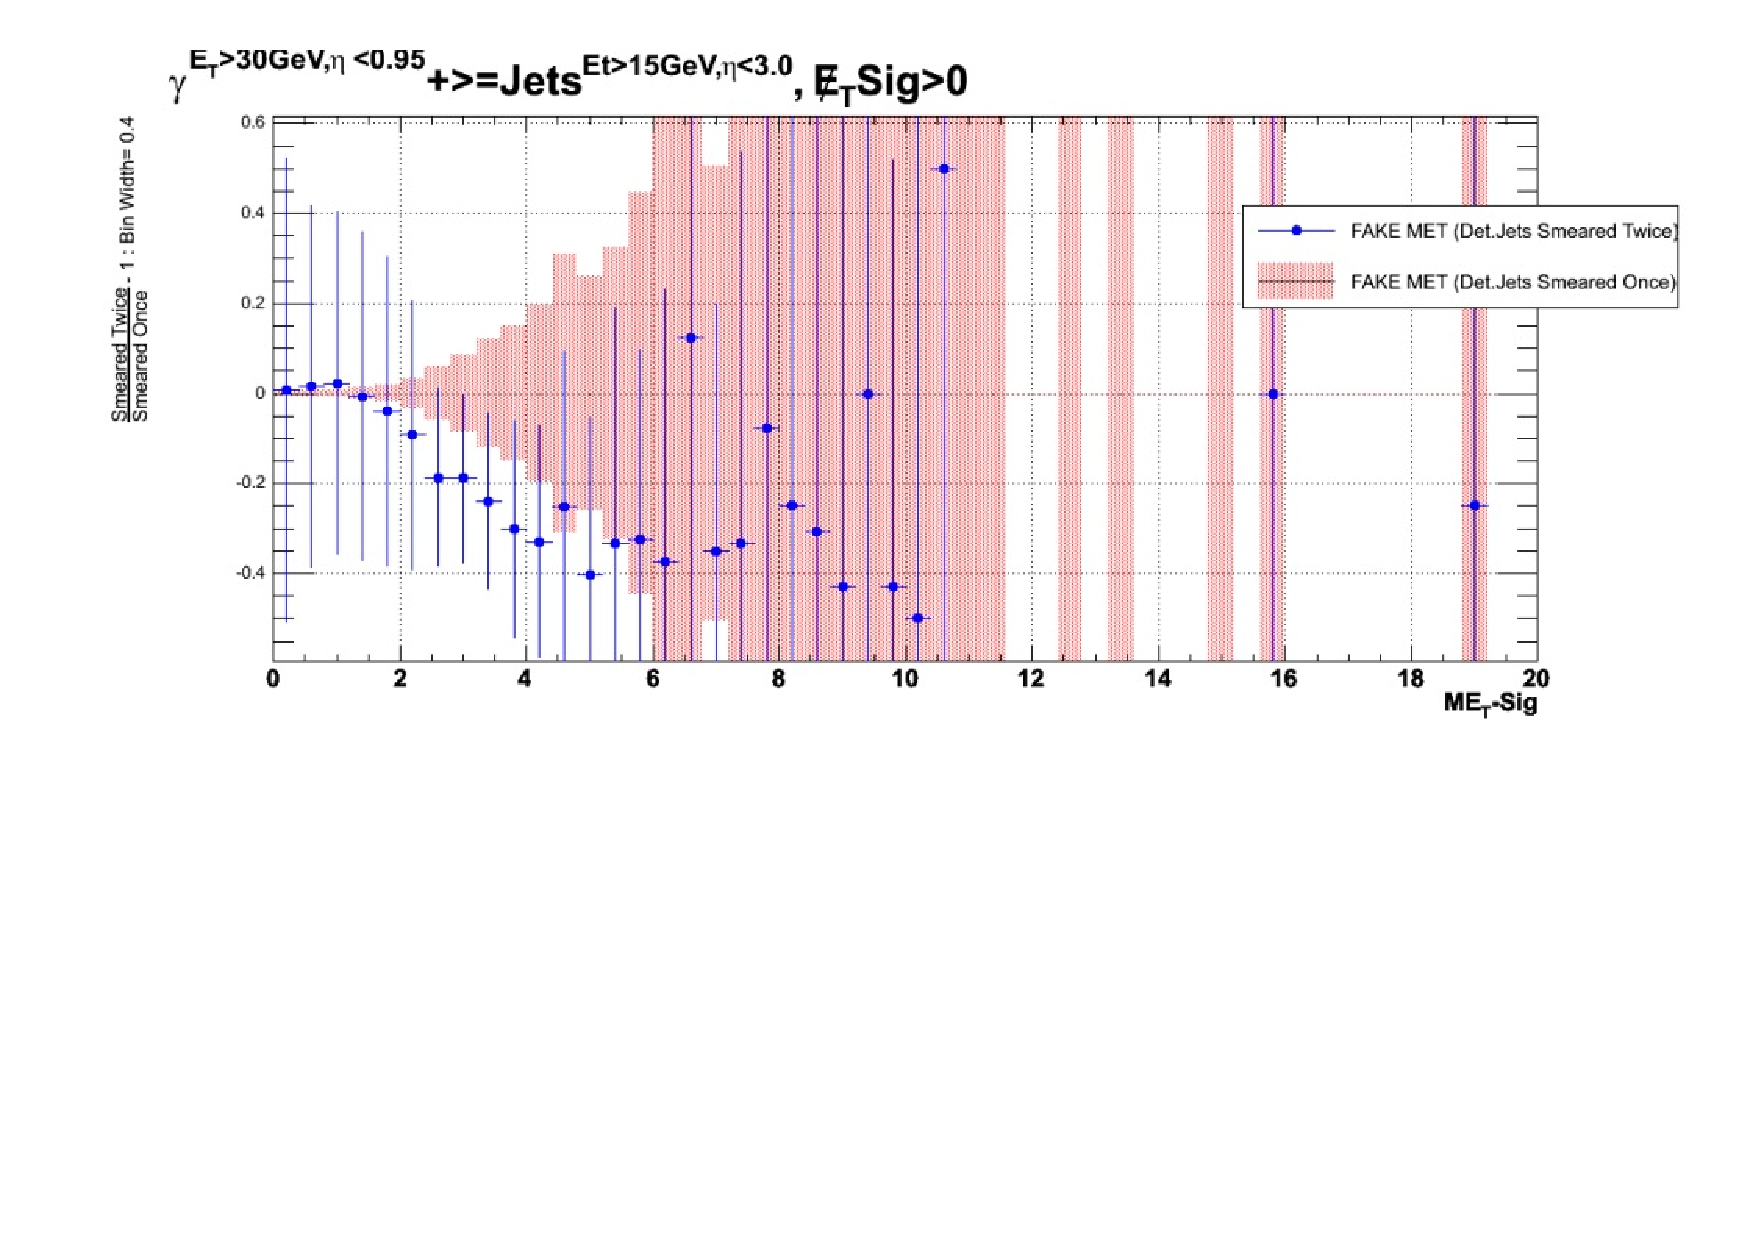
\includegraphics[scale=0.3,keepaspectratio=true]{./MetModel_DoubleSmear_MetSig.pdf}
% }
%
% \caption{Double smearing study of jet.}
% \label{fig:DoubleSmear}
% \end{figure}
%
%
% The results are inconclusive and require additional tests. And hence the standard method is used.)

\section{Preliminary Tests}
Numerous tests were performed to adopt the \met model for this photon + jets analysis in order to gain more sensitivity to physics beyond the Standard Model. Unlike other analyses that adopted the \met model for their \met measurement, it was difficult to adopt it for this analysis because it is dominated by jets. The \met measurement was not successfully modeled by the \met model, and even the \met-significance was discrepant.

We looked at exclusive photon + 1 jet events, and still some differences in the prediction of the \met model were seen. We also tested ways to add \met to jets before smearing them. We added \met to the leading jet and to the jet closest to the \met direction, and neither showed any significant improvement. Furthermore, we tested the addition of photon isolation energy back to the photon energy in order to improve the \met measurement. We also tried improving the parametrization of JER in the low \pt region. None of these led to a conclusive result or pointed to a solution. Further tests are needed to understand the behavior of the model with the presence of a large number of jets.

